
\section{Introdução}

\par Para a disciplina de \textbf{Projeto de \textit{Software}} seu objetivo é analisar as metodologias de desenvolvimento/gerenciamento de projetos ágil, visando uma melhora no uso do tempo de desenvolvimento e a própria agilidade no desenvolvimento do projeto.
\par De forma sucinta o movimento ágil é uma alternativa a gestão tradicional de projetos, as abordagem ágis nos tempos atuais vem sendo se suma importância e um divisor de águas para que um projeto ou \textit{software} se manter no mercado, pois cada vez esta um ambiente incerto e turbulento.
\par Segundo \citeonline{smartsheet}, os quatro valores do manifesto ágil são:

 \begin{enumerate}[label=\Roman{*}, ref=(\roman{*})]
   \item Indivíduos e interações mais que processos e ferramentas
   \item \textit{Software} em funcionamento mais que documentação abrangente
   \item Colaboração com o cliente mais que negociação de contratos
   \item Responder a mudanças mais que seguir um plano
 \end{enumerate}
 \par E desta maneira possuem os \textbf{doze} princípios do manifesto ágil, e que são:
\begin{asparaenum}
  \item Satisfação do cliente por meio do fornecimento contínuo e adiantado de software.
  \item Acomodação de mudanças de requisito durante todo o processo de desenvolvimento.
  \item Entrega frequente de software em funcionamento.
  \item Colaboração entre as partes interessadas do negócio e os desenvolvedores em todo o projeto.
  \item Apoio, confiança e motivação das pessoas envolvidas.
  \item Possibilidade de interações presenciais.
  \item Software em funcionamento é a principal medida de progresso.
  \item Processos ágeis para dar apoio a um ritmo de desenvolvimento consistente.
  \item Atenção aos detalhes técnicos e ao design aumenta a agilidade.
  \item Simplicidade.
  \item Equipes auto-organizáveis realizam ótimas arquiteturas, requisitos e designs.
  \item Reflexões periódicas sobre como aumentar a eficácia.

  \cite{smartsheet}
\end{asparaenum}

\par Esta aula prática tem por objetivo o desenvolvimento das etapa de um projeto hipotético ágil, com o fim de aplicar os conhcimentos adqueridos na cadeira de \textbf{projeto de \textit{software}}.

\section{Métodos}
\par Para o desenvovimento desta aula prática foi disponibilizado um roteiro, e segindo este roteiro é porposto elaboração em duas etapas, sendo elas:
\begin{enumerate}
  \item Se colocar no lugar do cliente, e pensar em um aplicativo para a confecção.
  \item E se colocar no lugar do \textit{product owner}, que deverá elaborar o aplicativo proposto.
\end{enumerate}


\noindent \begin{minipage}[c]{0.6\textwidth}
  \vspace {1cm}
\par Após as análises iniciais, o roteiro propõe o uso de algumas ferramentas para controle de etapas \textbf{(IceScrumm, Trello e Asna)}, opto pelo uso do \href{https://trello.com/home}{Trello}, esta ferramenta proporciona a integração com o \href{www.github.com}{GitHub}, adicionado e comentando ramificações e solicitações de mesclagem de fragmentos de códigos.

\end{minipage}
\begin{minipage}[c]{0.4\textwidth}
  \captionof{figure}{Logo Trello}
  
\includegraphics[width=\textwidth]{figure/trello.png}
  \label{fig:log_trello}
  {\fontsize{10pt}{\baselineskip} \selectfont Fonte: \citeonline{logtrello}}
\end{minipage}




\section{Resultados}
\par A eleboração desta aula prática esta dividida em duas partes, a primeira, no qual serei o cliente e deverá propor um aplicativo que se deseja desenvolver, levantar as funcionalidades e características.
\par Na segunda etapa, deverá ser o \textit{Product Owner}, quem ira desenvolver o aplicativo proposto e as responsabilidades desta etapa são:
\begin{itemize}
  \item Definir as funcionalidades do produto, ou seja, desenvolver o \textit{product backlog};
  \item Priorizar as funcionalidades de acordo com o valor de negócio;
  \item Montar um quadro do Scrum (Kanban) com as divisões de etapas, tarefas, data de entrega e responsáveis por atividade. Para este item, imagine que o desenvolvimento do seu aplicativo está em um estágio mais avançado, por este motivo, deve haver tarefas em todas as etapas. Utilize uma das ferramentas propostas para montar o seu quadro.
\end{itemize}

\subsection{Primeira etapa}
\par O aplicativo em questão deverá atender uma necessidade de geração de documentos personalizados, no qual o mesmo deverá ler tabelas em um arquivo com extensão .pdf \textit{Portable Documento Format}, o arquivo deverá posuir mais do que um tipo de documento gerado, deve ter a opção de escolher qual deseja gerar e os documentos deverão ser gerar para todos os nomes da tabela do arquivo pdf.
\begin{enumerate}
  \item Buscar o arquivo com extensão pdf mais novo na área de trabalho do usuário;
  \item Ler um arquivo pdf e extrair das tabelas os nomes e números de prontuários;
  \item Selecionar o modelo de documentos que serão gerados para todos os nomes com seus rescpectivos números de prontuários;
  \item Escolher se desejo imprimir e em qual bandeja;
  \item Escolher se desejo juntar os termo em um único pdf ou deixar em arquivos separados e salvar em uma pasta na área de trabalho.

\end{enumerate}\label{productlog}

\subsection{Segunda etapa}
\par Nesta etapa passo de cliente para desenvolvedor da solução, e para tal utiliza-se as feramentas de controle, versionamento de projetos e gerenciamento de projetos.


\subsubsection{\textit{Product backlog}}
\par O \textit{product backlog}, tem a finalidade de listar todas as caracteristicas, funções, requesitos e mudanças a futura que o produto precisa, pode se afirmar que o \textit{product backlog} \ref{productlog} ele não dever ser "apegado"\ pois cada vez que necessario deverá ser removido ou adicionado itens.
\par Trocando por miudos o \textit{product backlog} é uma lista de tarefas emplihada que deverá ser feito a cabeça primeiro e ir em direçã a sua caulda até concluir o desenvolvimento, sendo que a cabeça é a base para o software funcionar e em direção a caulda são melhorias do sistema que trará valor ao software. Na figura \ref{priorizacao-backlog}, podemos verificar um exemplo de \textit{product backlog}.
\begin{figure}[H] %Figuras da aula pratica 1.1
  \center
  \caption{Exemplo de \textit{product backlog}}

  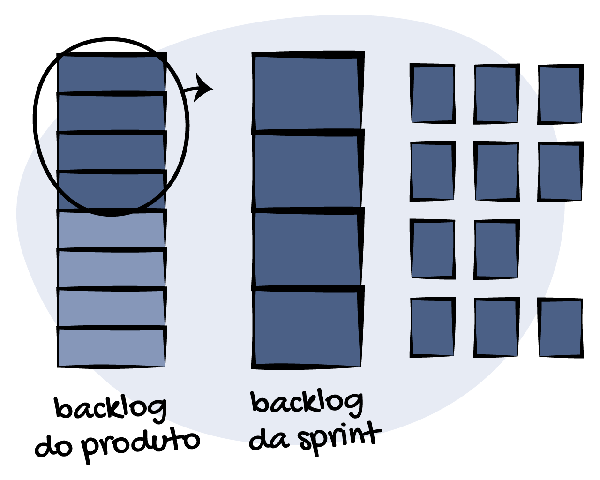
\includegraphics[width=\textwidth]{figure/priorizacao-backlog.png}
  % Deixar o espço

  \raggedright
  {\fontsize{10pt}{\baselineskip}\selectfont Fonte: \citeonline{kbn}}
  \label{priorizacao-backlog}
\end{figure}
%\href{https://odonodoproduto.com/backlog-do-produto/}{ver link}


\subsubsection{Quadro Kanban}
\par O quadro \textbf{Kanban}, representa um fluxo de tarefas o que paga um \textit{backlog} (Lista tarefas) e divide em sub tarefas e estas tarefas são organizadas em quadros do tipo: \textbf{A FAZER; FAZENDO e CONCLUIDO}, observa-se um exemplo na figura \ref{fig:kbn}. Na coluna \textbf{LISTA DE REQUISITOS}, seria o \textit{backlog} que posteriormente o mesmo é divido em sub tarefas e adicionado nas colunas \textbf{A FAZER; FAZENDO e CONCLUIDO}.

\begin{figure}[H] %Figuras da aula pratica 1.1
  \center
  \caption{Exemplo de quadro Kanban}

  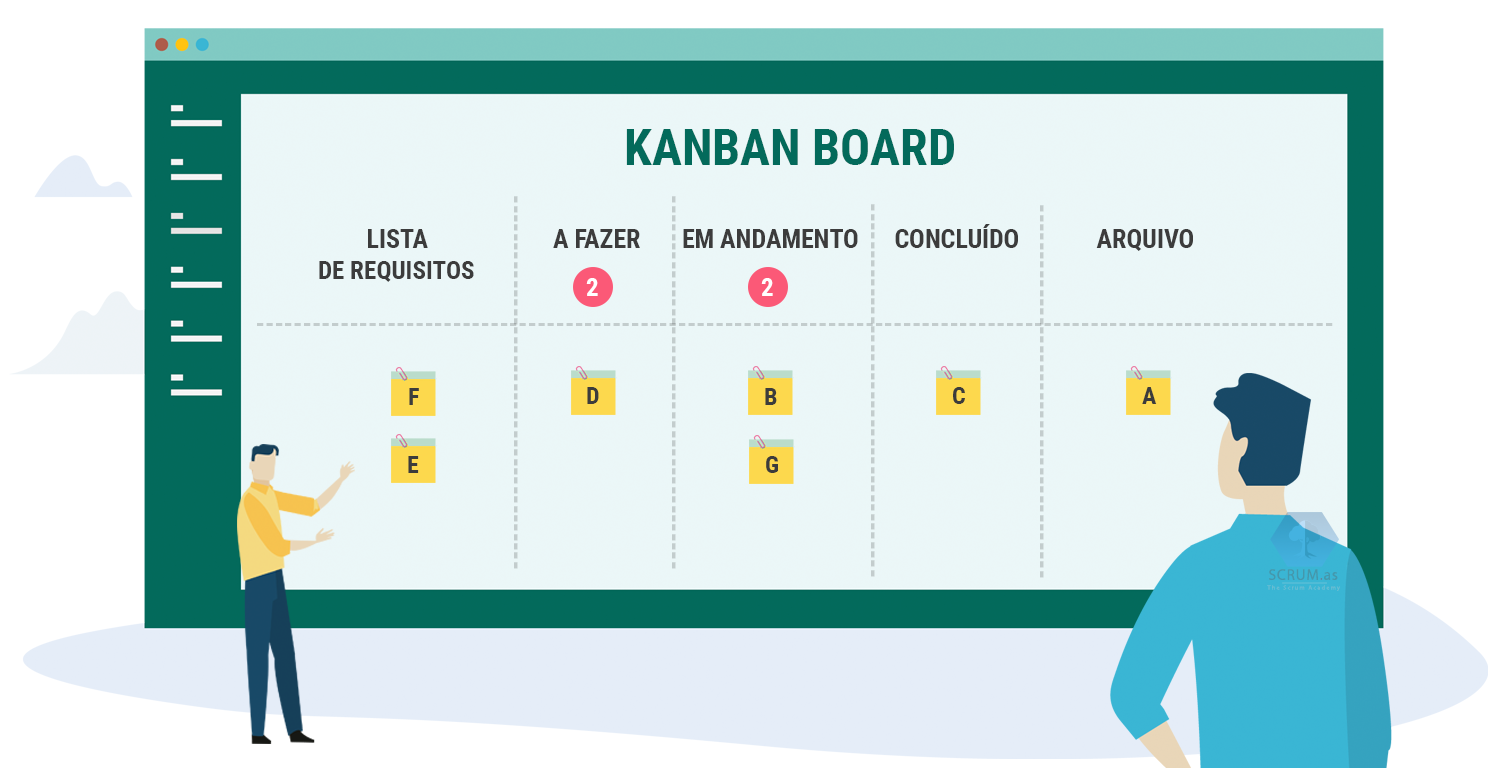
\includegraphics[width=\textwidth]{figure/kbn.png}
  % Deixar o espço

  \raggedright
  {\fontsize{10pt}{\baselineskip}\selectfont Fonte: \citeonline{kbn}}
  \label{fig:kbn}
\end{figure}


\par Deste modo prosseguimos para a elaboração do quadro \textbf{Kanban} da aula prática a qual pode ser observada na sequência das figuras \ref{fig:resultado}, o quadro \textit{Kanban} permite a inclusão de várias equipes de trabalho, porém nesta pratica é confeccionado para equipe única.

\begin{figure}[H] %Figuras da aula pratica 1.1
  \center
  \caption{Resultado da Aula prática}
  \subfigure[Quadro Geral.\label{fig:quadrokbn}]{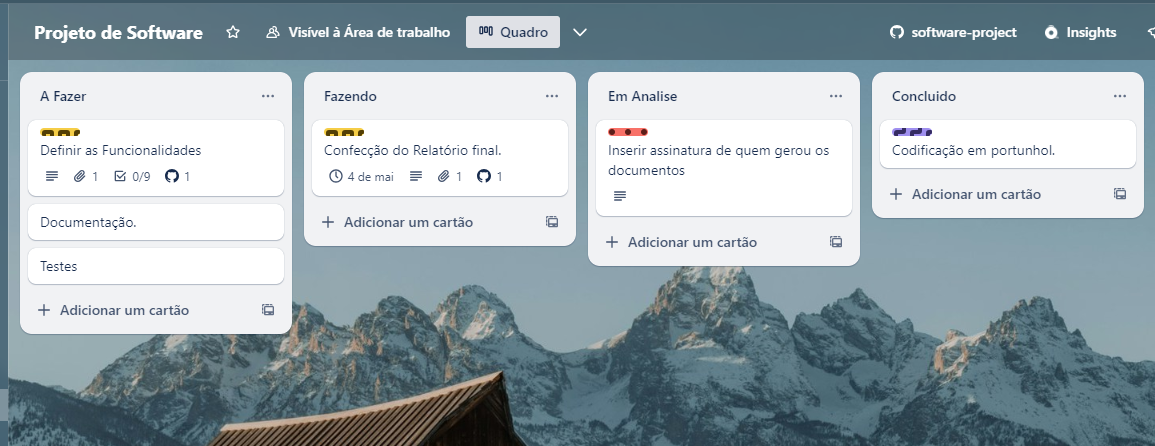
\includegraphics[scale=0.4]{figure/quadr.png}}\\
  \subfigure[Fragmento do quadro.\label{fig:seg2}]{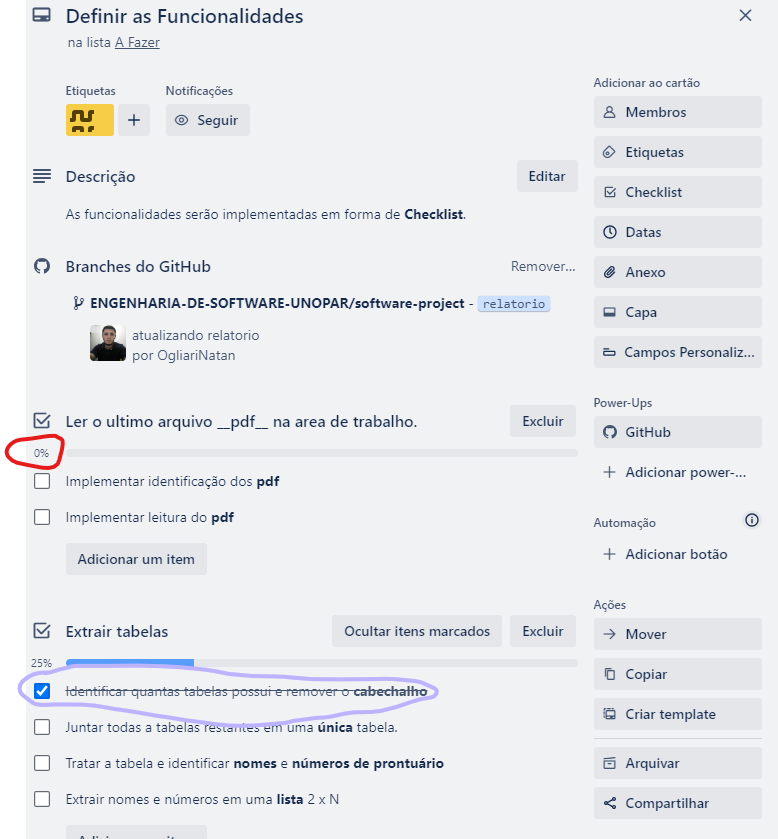
\includegraphics[scale=.4]{figure/frag1.png}}\\
  \subfigure[Registro de atividades com o Trello.\label{fig:seg3}]{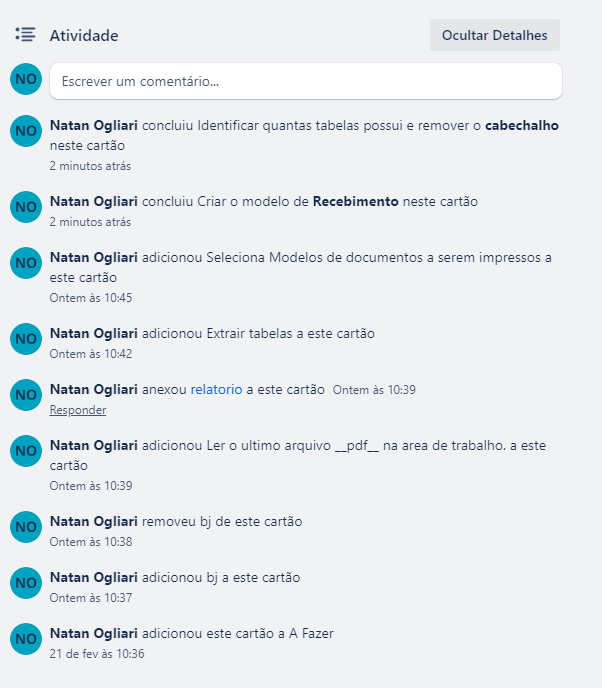
\includegraphics[scale=.4]{figure/log.png}}\\
  % Deixar o espço

  \raggedright
  {\fontsize{10pt}{\baselineskip}\selectfont Fonte: O autor (2024)}
  \label{fig:resultado}
\end{figure}


\par Com o uso do Trello\ref{fig:log_trello}, para esta aula prática evedencia as funcionalidades deste SaaS, como demonstrado na figura \ref{fig:seg2} o qual evedencia o usi de \textit{check list} e o percentual das sub tarefas desenvolvidas, já na figura \ref{fig:seg3} é possível verificaros registros de atividades relacionadas a tarefa em questão sem contar na integração com a plataforma GitHub conforme demonstrado na figura \ref{fig:gitgera}

\begin{figure}[H] %Figuras da aula pratica 1.1
  \center
  \caption{Resultado integração com GitHub}
  \subfigure[Integração GitHub.\label{fig:pri2}]{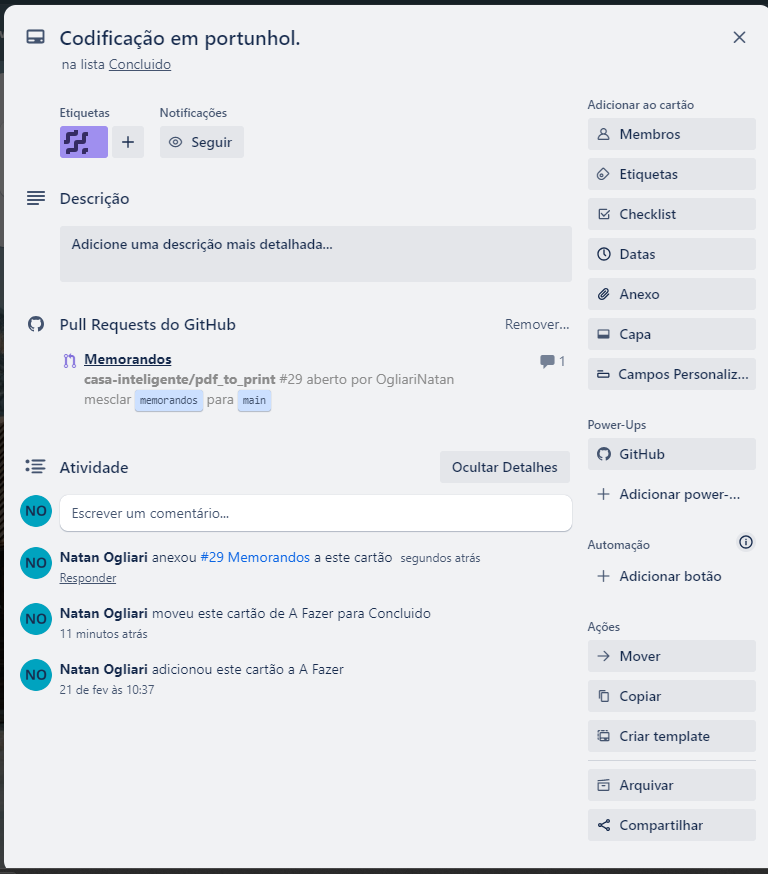
\includegraphics[scale=0.4]{figure/githu.png}}
  \subfigure[Integração GitHub.\label{fig:git}]{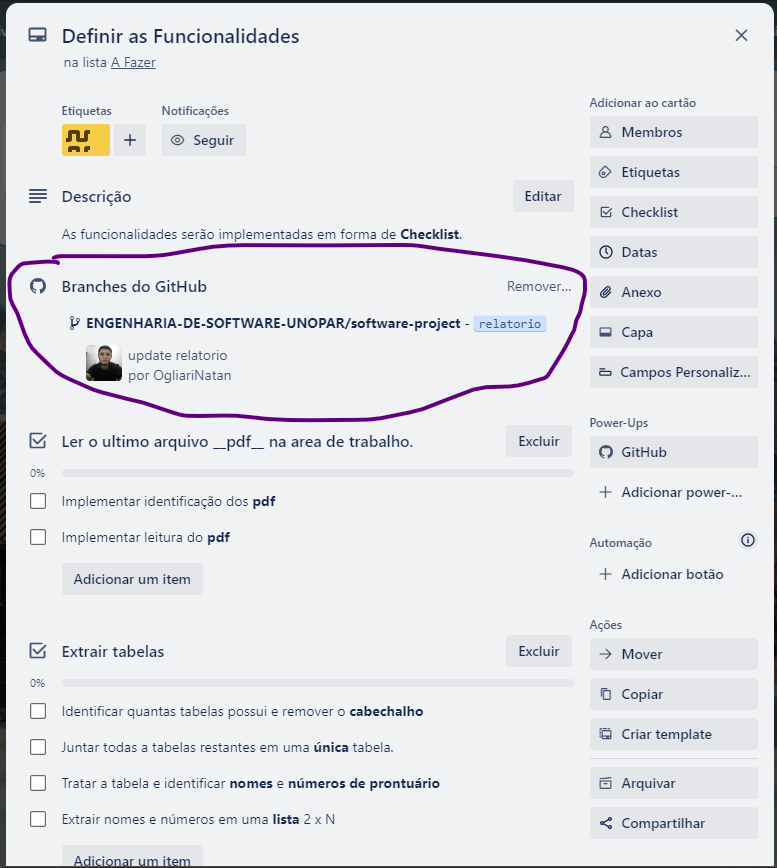
\includegraphics[scale=.4]{figure/intGit.png}}
  % Deixar o espço

  \raggedright
  {\fontsize{10pt}{\baselineskip}\selectfont Fonte: O autor (2024)}
  \label{fig:gitgera}
\end{figure}


%\par Estou usando \href {https://cocalc.com/} {CoCal}

%E para referenciar a figura \ref{fig:imagem_massa} utilize dessa forma. \LaTeX






\section{Conclusões}

\par Podemos aferir com elaboração da aula prática, a necessidade do uso de metodologias na gestão de software, não possui apenas um tipo de gestão, pelo contrario possui inumeros e todos com a funcionalidade de desenvolvimento agil. Suas implementação são trabalhosas e demandam conhecimento e prática, é por estes e outros= motivos que no mercado atualmente possui cargos expecifico para gerente de projetos.



  %$X \xLongleftarrow[\text{NATAN}]{\text{OGLIARI}} Y $ %COM TEXTO
	% $\uparrow$ %Seta para Cima
	%$\overleftarrow{NATAN}$
